\chapter{Design and Specification}\label{ch_method}

\section{Aim/vision}

The idea of the game is to travel around the world without physically
having to be there, inviting the user to realise the scale of the
world whilst gaining the positive benefits of outdoor exercise. A user
may decide to run around areas in Scotland (the Scotland Mission) and
this is achieved through routes such as Glasgow to Edinburgh. Each
route is further broken up into manageable stages of a few kilometres
and users are awarded badges based on stages/routes completed and
overall distance and time. Therefore the user can gain short-term
success while working towards the satisfaction of larger goals. 

This approach is to test whether or not this type of encouragement
could potentially work with outdoor exercise. Metrics will be tracked
for individual users to monitor their exercise duration and frequency
and will be used to encourage that user to exercise. These metics will
then be used to form the basis of our conclusion.



The physical aims of the project are then as follows:

\begin{enumerate}
  \item To provide incentives that become intrinsically
    rewarding. Rewards are primarily linked to stage and route 
    completion and these accumulate to the completion of the entire
    mission - every achievement brings the user closer to a larger
    success. 
  \item To provide long and short term goals to fulfil the sense of
    achievement. The long term goals are Missions which are achieved
    through the medium term goals of Routes and easily achievable
    short term goals of Stages - for example
    the Scotland Mission has a Glasgow to Edinburgh Route which has a
    Falkirk to Linlithgow Stage.
    \begin{enumerate}
      \item Stage completion - unlock a photograph of the stage or of
        a key landmark near the stage. This is achieved by completing
        a specific stage.
      \item Route Completion - stamp in the travel book for that
        mission relating to route completed. This is achieved by
        completing all the stages in the route.
      \item Mission Completion - travel book for mission is
        ``framed'', certifying that the user has completed all routes
        in the mission.
    \end{enumerate}
\end{enumerate}


\section{Specification}
\subsection{N-Tier Diagram}
The high level components of this system are reasonably simple (figure
\ref{NTier}). The
user requires a mobile phone with GPS enabled and the mobile
application installed. This communicates with a Django Webserver with a
REST-style API (with a small number of bespoke views since some
behaviour does not fit well with the REST specification) which in turn
uses Django's Object Relation Model (ORM) to persist these to a
database.

The mobile application communicates with the devices GPS location
management system to get accurate location information for the
user.
\begin{figure}[h]
  \centering
  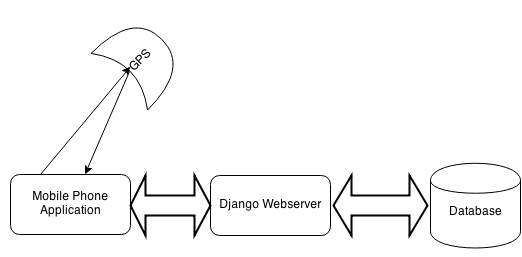
\includegraphics[width=\linewidth]{images/N-tier.png}
  \caption{N-Tier diagram}
  \label{NTier}
\end{figure}

\subsection{Entity Relation Diagram}
\label{sec:ER}
There have been two significant iterations of the Entity Relation (ER)
diagram in this project - the first is the final theoretical ER model
and the second is the real world implementation with modifications and
extra linking for data transfer optimisation. 

The main reason for the implementation modifications is to keep data
transfer low between the mobile device and the API. Since the mobile
device will be using non-wifi based communication methods the number
of bytes transferred will be logged by their network provided and will
cost the end user. The application requires many data objects of the
same type (when picking a route to travel down from a list of all
routes for example) so it makes sense to bundle all all the requests
into one and reduce the data transfer overhead. 

\begin{figure}[h]
  \centering
  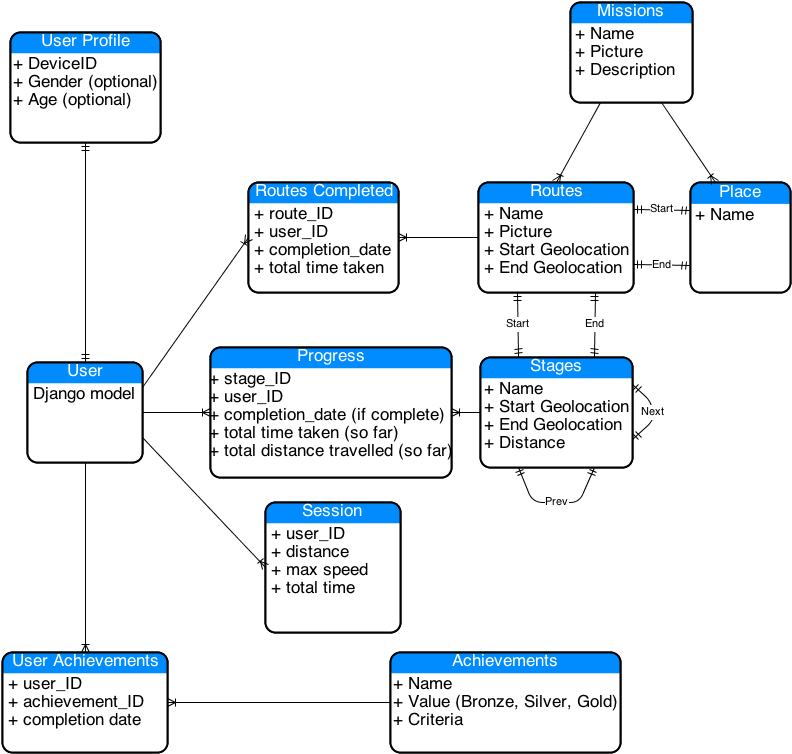
\includegraphics[width=\linewidth]{images/ER.png}
  \caption{ER diagram, final theoretical model}
  \label{ER_1}
\end{figure}

\todo{Do implementation ER diagram}

\subsection{Platform}
The mobile application is developed using PhoneGap which packages a
web app into mobile app. The decision to use PhoneGap instead of
building a native app is primarily because I come from a web
development background but also so we can deploy to multiple platforms easily
without needing to change the code base.

The web application is written in Python and uses Django middleware
for interfacing with the database and creation of specific workflow
interactions, alongside Tastypie for managing and building a REST
style API.

The server will not hold state outside the supporting database and
will be used solely as a REST API. This is a decision to keep the
sever implementation clean and simple. There is also no real gain to
maintaining state as the underlying database objects all ready hold
the required information.

\subsection{Walkthrough of Wireframes}
\begin{figure}[h]
  \centering
  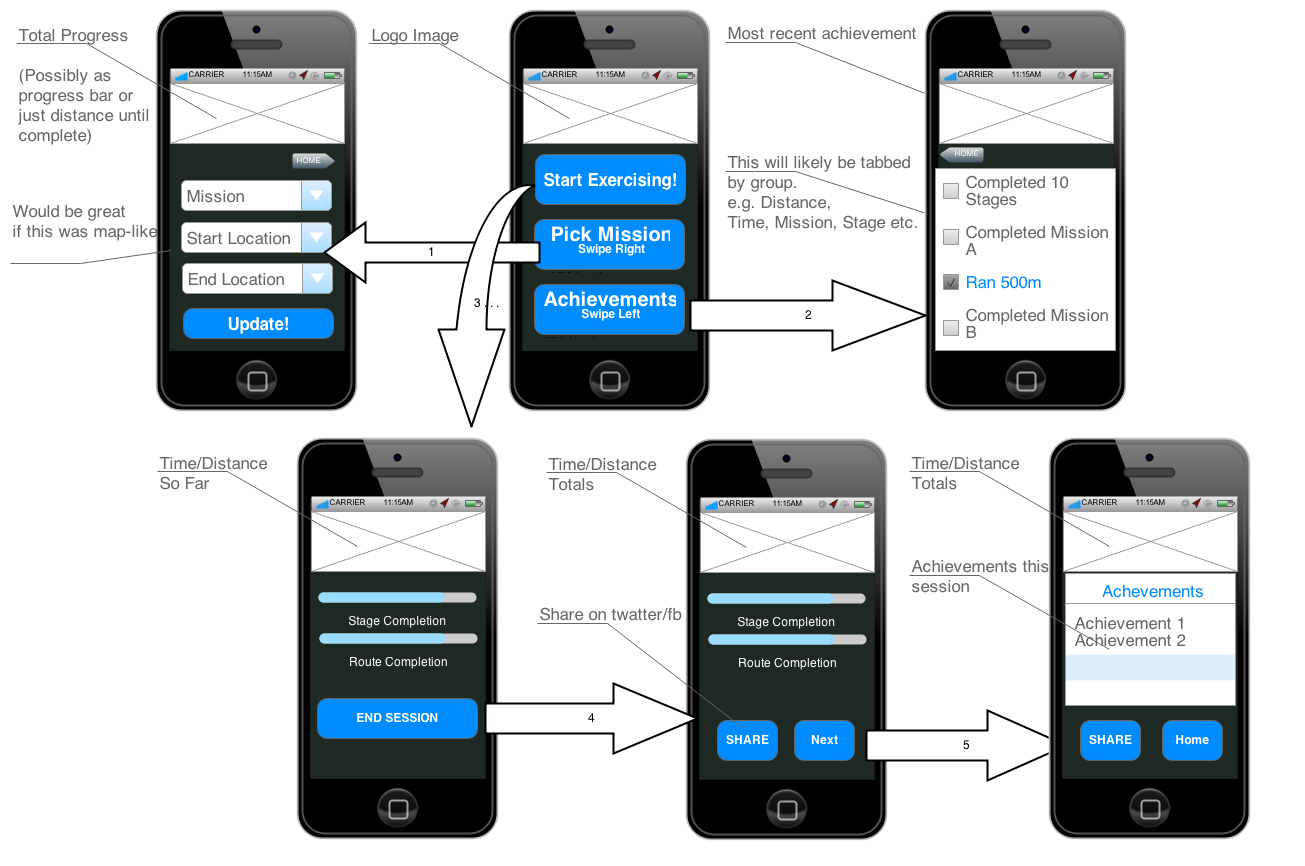
\includegraphics[width=\linewidth]{images/Wireframes.png}
  \caption{Wireframes, initial design}
  \label{wireframes_1}
\end{figure}

When the app is launched it silently registers with the server
allowing the user to use the app immediately. The user is then shown
the middle-top screen.
\begin{enumerate}
\item From the middle top screen, the user can follow arrow 1 by
  clicking on the middle button ``Pick Mission'' to pick a Mission
  (Run around Arran or Egg for example) and then pick a start and
  end location. After confirming these choices, the user is taken
  back to the middle top screen, or at any time can click the
  ``Home'' button to return. 
\item The user can also view their current acheivements by clicking
  the ``Achievements'' button on the middle top screen, following
  arrow 2. These achievements will be grouped by tabs by category -
  Distance, Time, Stage and Mission based achievements.
\item The user can follow arrow 3 from the middle top screen to
  notify the app that they are starting an exercise period, telling
  the app to track their distance. If a Mission and start and end
  location are not picked (as in point 1) then they will instead be
  redirected to this screen and are unable to start exercising until
  this choice has been made. Once they have successfully advanced to
  this screen, it will display their current progress as they move
  showing the user how close to completion of their current stage
  and overall route they are. 
\item When the user has finished exercising, they will click the
  ``End Session'' button and be taken to the first summary screen -
  following arrow 4. Here statistics from their exercise will be
  shown and the option to share this on several social media
  outlets.
\item The user can then move to the second and final summary screen,
  following arrow 5, where they will be shown any achievements they
  were awarded during that session. The user will also have the
  option to share these on social media outlets. From here, the user
  can click the ``Home'' button and be taken back to the middle top
  screen. 
\end{enumerate}

\section{Notable design decisions}
\subsection{Explicit caching}
As was mentioned in Section \ref{sec:ER}, the minimisation of network
traffic is of great consideration when dealing with mobile devices. I
did not want the mobile device to make repeated API calls for
resources that will not change in the short term - resources such as
what missions are available, what routes belong to what missions and
what stages belong to each route. 

The main case for this is as follows. A user may open the app for the
sole purpose of browsing all missions and their routes, and any
progress they have on these routes before they start using the app for
exercise. In an unmanaged situation the app could call the API each
time it lands on a menu to pick a mission or the routes for a mission
- if the user is browsing then they may see the same information
provided several times. 

If we remove data transfer from the equation all together and focus
solely on the user experience then caching will give a better user
experience in terms of loading speed. Since caching means we do not
have to hit the API each time we want to see something we have seen
before, we can load selection menus faster. 

Note that I only intend to cache data endpoints that are unlikely to
change in the short term or those that cannot feasibly change in a
situation like this. The ``progress'' endpoint which provides the data
about a users progress along given stages will not change if the user
does not initiate an exercise session as there is no data provided to
show otherwise. 

These caching services are used as singleton-like facilities in the
application to ensure consistent data throughout the application, and
also to allow the addition of new data from any point in the
application and use that new data in a different part at a later time.

\subsection{Exercise Session Management}
Due to the environmental implications brought on by GPS, a user may
drop out of connection for finding their location. The user should not
be penalised for this as it is outwith their control and is not a
direct error on their part. Something as simple as running through a
tunnel could initiate the loss of signal. 

To counter this, I have designed the exercise session object (herein
referred to as just a ``session'') to accommodate for this.

When a user decides to exercise, a new session is created through the
API. The users device is then given a unique ID for that session that
only they have a knowledge of (in the first iteration of this
implementation this ID is a direct mapping to the ID of the object in
the database, but in a future version this could be something more
obscure). Only this user can update this session and it can only be
updated if you know hte unique ID for that session. 

When you have a GPS location and are ready to update, you know the
unique ID and are able to update the session. If you do not have a GPS
location, then as long as you are still polling for a GPS location the
app will hold onto that unique ID so when you eventually get a GPS
location you can update easily.

The method for updating handles completion of many stages. This
implies that if you update a session and the stage you are currently
exercising on completes you will be immediately moved onto the next
stage on the route, if one is available. This also handles a use case
where you drop out of GPS connection and travel far enough to complete
more than one stage on the route you are on. Then the method will log
your progress on your last known stage, completing it, and then will
complete as many of the next stages as are available and that you have
enough accumulated distance to complete.

When you end the exercise session or close the app, the unique ID for
the session you are on is lost and so cannot be updated. This
effectively ``ends'' the session without explicitly doing so.

This should allow the user to drop in and out of GPS connection
without being penalised for doing so.

\subsection{Distance Verification}

\todo{Need to actually implement this}
